\documentclass[10pt,a4paper]{article}
\renewcommand{\baselinestretch}{1.0}
\usepackage{cite}
\usepackage[dvips]{graphicx}
\usepackage{psfrag}
\usepackage{color}
\usepackage[cmex10]{amsmath}
\usepackage{amsfonts}
\usepackage[font=footnotesize, captionskip=10pt]{subfig}
\usepackage{tikz}
\usepackage{flushend}
\usepackage{times}
\usepackage[margin=1.5cm]{geometry}
\usepackage[slovak, english]{babel}
\usepackage[utf8]{inputenc}
\usepackage[T1]{fontenc}
\usepackage{hyperref}

\usepackage{multirow}
\usepackage{colortbl}

\pagestyle{empty}

\hyphenation{net-works}
\newtheorem{remark}{Remark}

\begin{document}

\title{Playing multiple games using deep reinforcement learning, or Spatial Attention network can play (beat) simultaneously multiple games in reinforcement learning}
\author{Michal Chovanec, Katarína Jasenčáková, Katarína Bachratá, Hynek Bachratý}
\date{}
\maketitle
\thispagestyle{empty}

{\bf Abstract}
In this paper we presents deep Q network (DQN) playing multiple games with the same weights - six ATARI games.
We trained network by randomly changing games after several interations, using deep reinforcement learning.
For comparison, we also trained common DQN (one network per game). Our networks architectures are : basic convolutional neural network (CNN), DenseNet and Spatial Attention CNN.
Spatial Attention Network was able to outperform both (basic and DenseNet, with much fewer parameters than DenseNet).
Instead of using 8x8 or 4x4 kernels as in \cite{bib:dqn_atari} and \cite{bib:dqn_doom}  we used only 3x3 kernels, and much lower of feature maps in layers.
Presented networks are much more parameter and computation cost effective. As results we present training score progress, network feature kernels maps for each game and attention heatmaps.


\section{Introduction}


\begin{figure}[htb!]
\centering
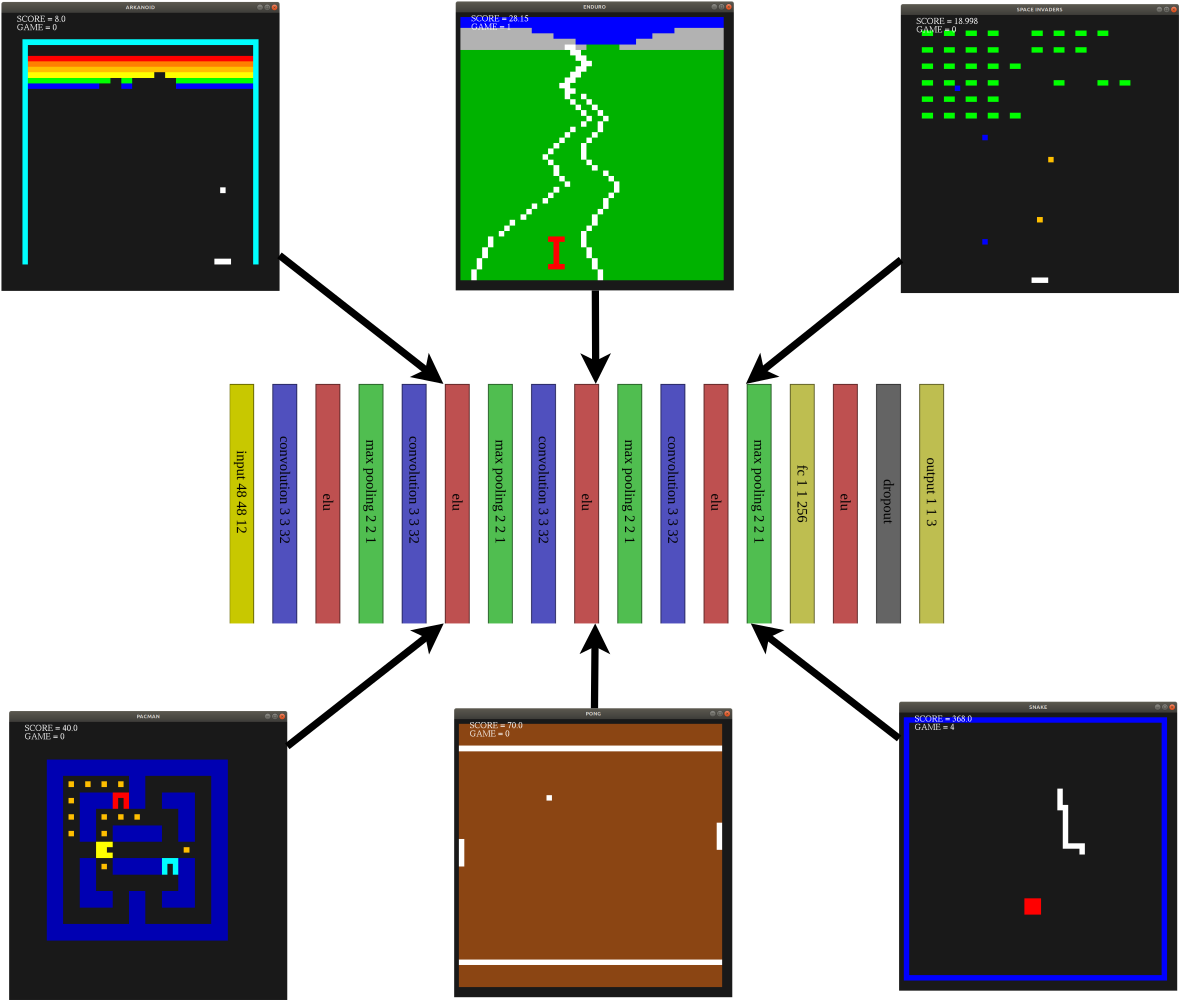
\includegraphics[width=0.5\textwidth]{diagrams/multi_dqn.png}
\caption{Multi DQN can play six games with the same weights}

\end{figure}

\newpage
\section{Experiment setup}

We choosen 6 Atari games, in 48x48 grid : Arkanoid, Enduro, Invaders, Pacman, Pong and Snake.
For relevant results, we first trained 6 basic CNN, each for one game. We choosen 1000 games for training and 100 games for testing the final score.
Then we trained three different architectures (named multi\_net\_0 ... 2). Those networks have different architectures (basic CNN, DenseNet and Spatial Attention CNN).
During training, the games were randomly changed (after 8192 iterations). Training is finished when there are played 1000 games from all games,.
As input (game state) into neural network we used raw frame stacking. Our input are last four RGB frames, with size 48x48 pixels. This leads to input tensor dimensions of 48x48x12 or 48x48x3x4 if
4D tensors are used. Outputs are linear mapped Q values on last network layer.
For action selecting we choosen $\epsilon$-greedy strategy. Starting on $\epsilon = 1$ (total random strategy) exponentialy decreasing to value $\epsilon = 0.1$.

\subsection {Network architecture}
Following state of the art \cite{bib:vgg_net} and \cite{bib:resnet_net}, we used only 3x3 kernels with stride 1, instead of 8x8 kernels as in \cite{bib:dqn_atari}.
As activation function the ELU is choosen, with $\alpha = 0.1$. After convolution and pooling layer we used one full connected with 256 units and second
full connected corresponding to actions count in game. For multi\_nets the amount of units on last layer depends on game with maximum possible actions.

{\bf Basic network architecture}:
multi\_net\_0 is basic deep Q network - the same as individual games playing networks.
There are four convolutional layers with 32 filters, followed by ELU activation, 2x2 pooling and one 256 units full connected layer.
The last layer with linear activation is directly mapping outputs to Q values. Number of units on this layer is equal to actions count
(respectively maximum required actions - in our case it is 5).
We also tried network without 256 FC layer - to reduce amount of parameters, but the training was much slower \footnote {We are not presenting results, but this require more research - how to reduce number of parameters in DQN and make training faster}.

{\bf DenseNet network architecture}:
Next tested architecture is DenseNet \cite{bib:densenet_net}, multi\_net\_1. We used four dense blocks. Each dense block consist of four 3x3x32 convolutional layers, one 1x1x32 layer and 2x2 pooling layer.
The main idea is to use state of the art network, which have much bigger capacity and probaly can outperform basic DQN. The main problem can be a lot
of parameters of this network. Thanks dense connection, the much deeper architecture can be used, and much more complex features can be extracted.

{\bf Spatial Attention CNN network architecture}:
The last architecture we tested is Spatial Attention CNN, inspired by \cite{bib:cbam}, multi\_net\_1.
The main idea of attention in CNN is to "amplify" some selected featured and present them to next layer.
Our presented attention module is illustrated on figure \ref{img:spatial_attention_module}.
Input tensor with dimensions $width \times height \times depth$ is processed in convolution block (with kernel size $3 \times 3 \times depth$).
Instead of input features-depth pooling - which is useful in classification attention networks, we are using full features inputs into convolution module (layer).
After convolution the sigmoid non-linear activation is applied on feature maps. Next block is gating unit, which is using point-wise (Hadamard) product.
The last step is addition block, which adds original input and attention features - this can be intepreted as ResNet idea. Full network architectures can be seen in table \ref{tab:networks}.
The formal definition can be written in following term

\begin{align}
y = x + x \odot f(x; w, b)
\end{align}

where \\
$x$ is input tensor \\
$y$ is output tensor \\
$w$, $b$ are kernel weights and bias respectively \\
$f(x; w)$ is convolution between x and w followed by sigmoid nonliearity.

\begin{figure}[htb!]
\centering
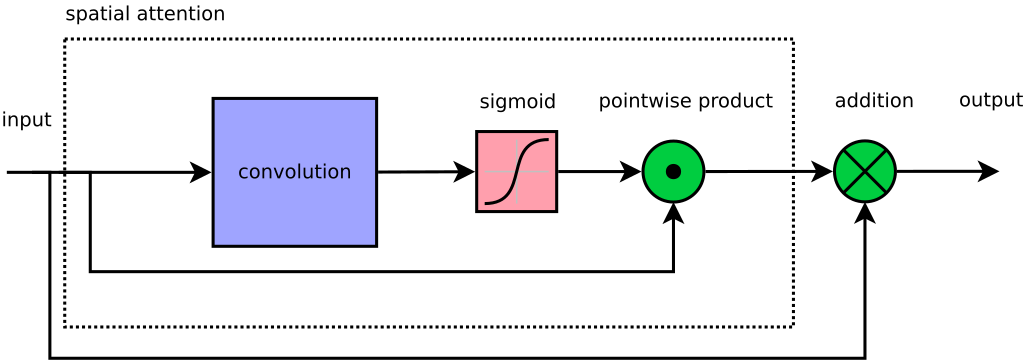
\includegraphics[width=0.5\textwidth]{diagrams/spatial_attention.png}
\caption{Designed spatial attention module}
\label{img:spatial_attention_module}
\end{figure}

We choosen the some hyperparameters for all networks. Only difference is minibatch size. For single game playing net we choosen size 32, for multi-nets 128 - to chieve better
training stability. Summary hyperparameters setup are :
\begin{itemize}
    \item learning rate $\eta = 0.001$
    \item L1 and L2 regularization $\lambda _1 = \lambda _2 = 0.0000001$
    \item dropout $0.02$ (only after FC256 layer)
    \item minibatch size 32 for single DQN, 128 for multi DQN
    \item gradient clip $\langle -10, 10 \rangle$
    \item Q-learning discount factor $\gamma = 0.99$
\end{itemize}



% Please add the following required packages to your document preamble:
% \usepackage[table,xcdraw]{xcolor}
% If you use beamer only pass "xcolor=table" option, i.e. \documentclass[xcolor=table]{beamer}
\begin{table}[htb!]
\centering
\begin{tabular}{|l|l|l|l|}
\hline
\textbf{layer} & \textbf{multi\_net\_0}             & \textbf{multi\_net\_1}                    & \textbf{multi\_net\_2}                \\ \hline
0              & \cellcolor[HTML]{CBCEFB}C3x3x32    & \cellcolor[HTML]{FFCCC9}4 x dense C3x3x32 & \cellcolor[HTML]{CBCEFB}C3x3x32       \\ \hline
1              & \cellcolor[HTML]{9AFF99}P2x2       & \cellcolor[HTML]{CBCEFB}C1x1x32           & \cellcolor[HTML]{6AFFFA}attention 3x3 \\ \hline
2              & \cellcolor[HTML]{CBCEFB}C3x3x32    & \cellcolor[HTML]{9AFF99}P2x2              & \cellcolor[HTML]{9AFF99}P2x2          \\ \hline
3              & \cellcolor[HTML]{9AFF99}P2x2       & \cellcolor[HTML]{FFCCC9}4 x dense C3x3x32 & \cellcolor[HTML]{CBCEFB}C3x3x32       \\ \hline
4              & \cellcolor[HTML]{CBCEFB}C3x3x32    & \cellcolor[HTML]{CBCEFB}C1x1x32           & \cellcolor[HTML]{6AFFFA}attention 3x3 \\ \hline
5              & \cellcolor[HTML]{9AFF99}P2x2       & \cellcolor[HTML]{9AFF99}P2x2              & \cellcolor[HTML]{9AFF99}P2x2          \\ \hline
6              & \cellcolor[HTML]{CBCEFB}C3x3x32    & \cellcolor[HTML]{FFCCC9}4 x dense C3x3x32 & \cellcolor[HTML]{CBCEFB}C3x3x32       \\ \hline
7              & \cellcolor[HTML]{9AFF99}P2x2       & \cellcolor[HTML]{CBCEFB}C1x1x32           & \cellcolor[HTML]{6AFFFA}attention 3x3 \\ \hline
8              & \cellcolor[HTML]{FFFC9E}FC 256     & \cellcolor[HTML]{9AFF99}P2x2              & \cellcolor[HTML]{9AFF99}P2x2          \\ \hline
9              & \cellcolor[HTML]{FFFC9E}FC actions & \cellcolor[HTML]{FFCCC9}4 x dense C3x3x32 & \cellcolor[HTML]{CBCEFB}C3x3x32       \\ \hline
10             &                                    & \cellcolor[HTML]{CBCEFB}C1x1x32           & \cellcolor[HTML]{6AFFFA}attention 3x3 \\ \hline
11             &                                    & \cellcolor[HTML]{9AFF99}P2x2              & \cellcolor[HTML]{9AFF99}P2x2          \\ \hline
12             &                                    & \cellcolor[HTML]{FFFC9E}FC 256            & \cellcolor[HTML]{FFFC9E}FC 256        \\ \hline
13             &                                    & \cellcolor[HTML]{FFFC9E}FC actions        & \cellcolor[HTML]{FFFC9E}FC actions    \\ \hline
\end{tabular}
\caption{Tested networks architectures}
\label{tab:networks}
\end{table}






\newpage
\section{Results}

First we presents training score progress. The games rewards has been chosen to
be impossible achieve positive score only by random playing. On figures \ref{img:score_result} we
can see typical RL training progress - first is agent playing randomly, taking negative rewards.
After few hundred games the agent finds good strategy and is able to achieve more and more positive
rewards.

As second part, we focused on learned features visualisation. We processed the maximum kernel response, for
all networks and all kernels. The inputs for maximum kernel response are presented on figure \ref{img:max_response}.
Those images are obtained by maximizing kernel response using gradient backpropagation, starting with random input (cite). We
visualised only convolutional layers.

To compare trained networks for learning similar features we computed correlations between networks (TODO more specify how).
Considering networks features correlation (Table \ref{tab:networks_correlation}) we assume that
multi\_net\_0 is learning different features. But we can see strongest correlation with most complicated games - Pacman and Snake,
and the lowest correlation with the simplest game - Pong \footnote{most/less complicated game - in meaning of input complexity}.

This results leads us to visualise activation heatmap - to understand what are different networks focusing on.

\begin{figure}[htb!]
    \centering
    \subfloat[Arkanoid]{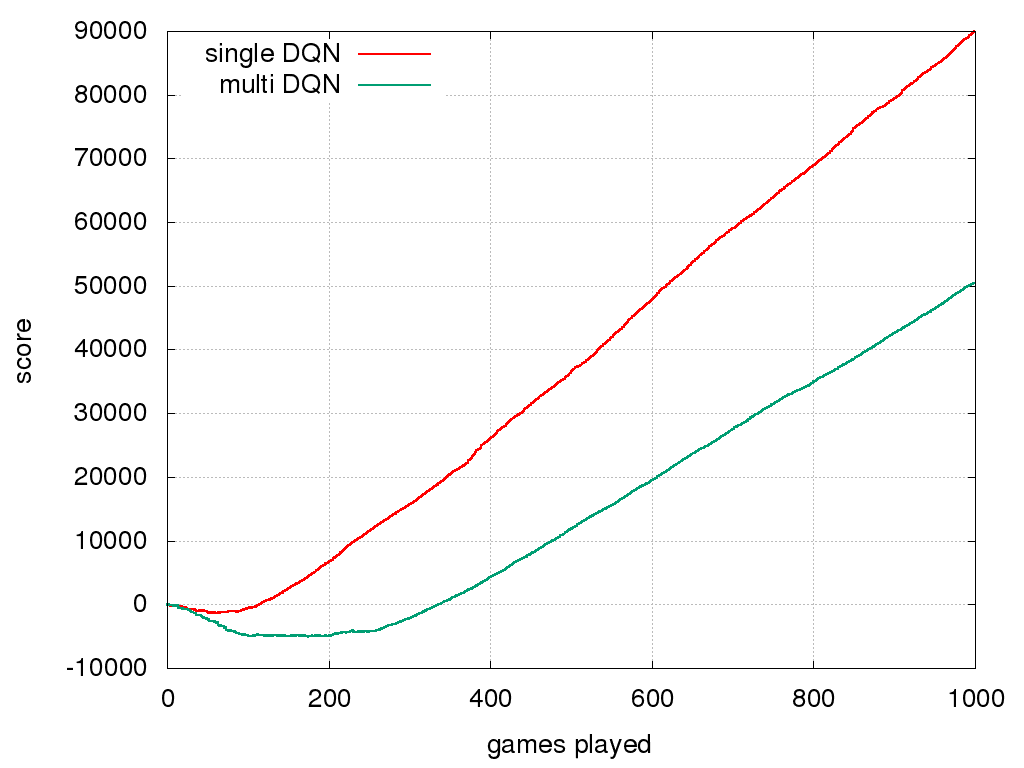
\includegraphics[width=5cm]{results/progress_training_arkanoid.png}}\hfil
    \subfloat[Enduro]{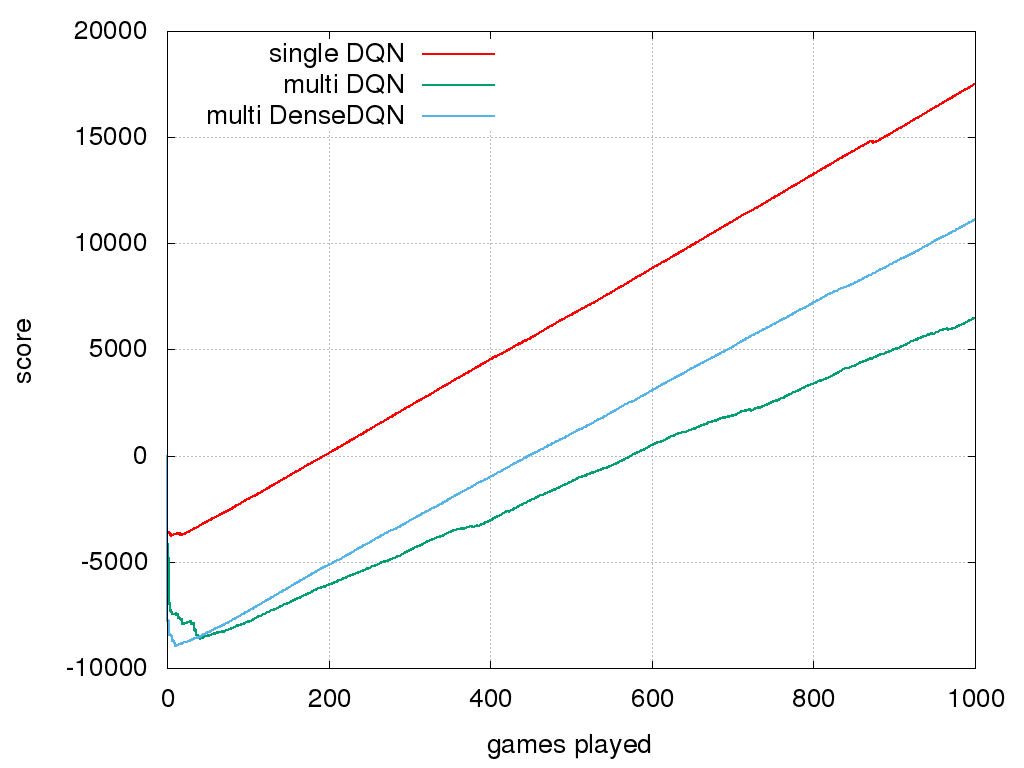
\includegraphics[width=5cm]{results/progress_training_enduro.png}}\hfil
    \subfloat[Invaders]{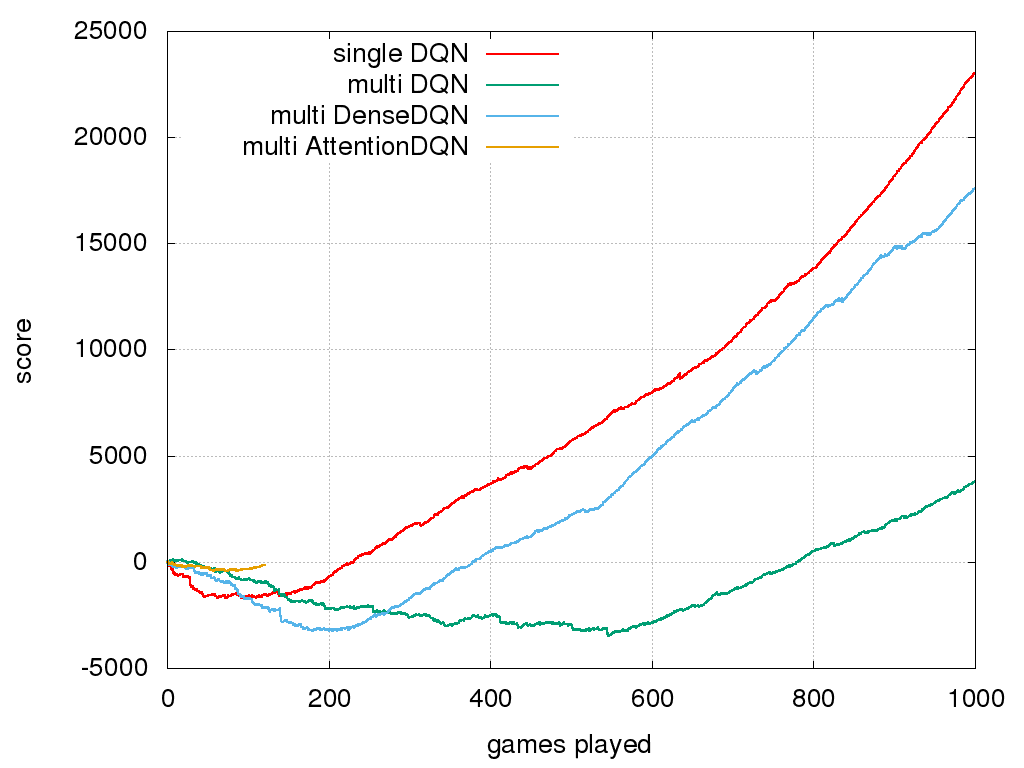
\includegraphics[width=5cm]{results/progress_training_invaders.png}}

    \subfloat[Pacman]{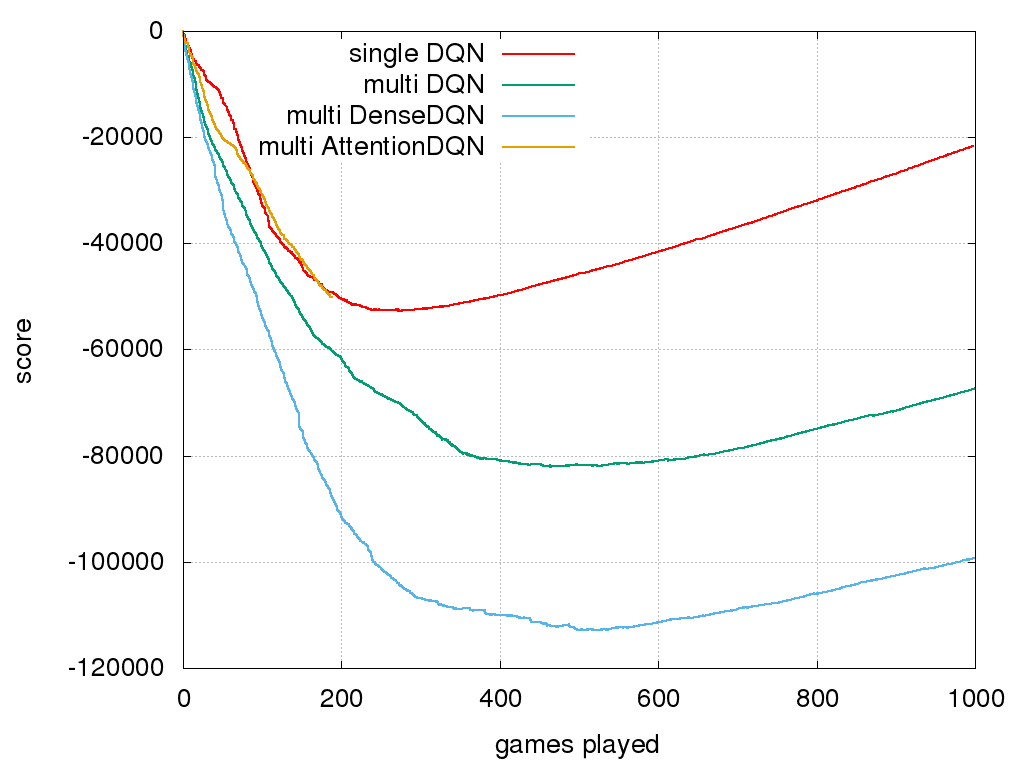
\includegraphics[width=5cm]{results/progress_training_pacman.png}}\hfil
    \subfloat[Pong]{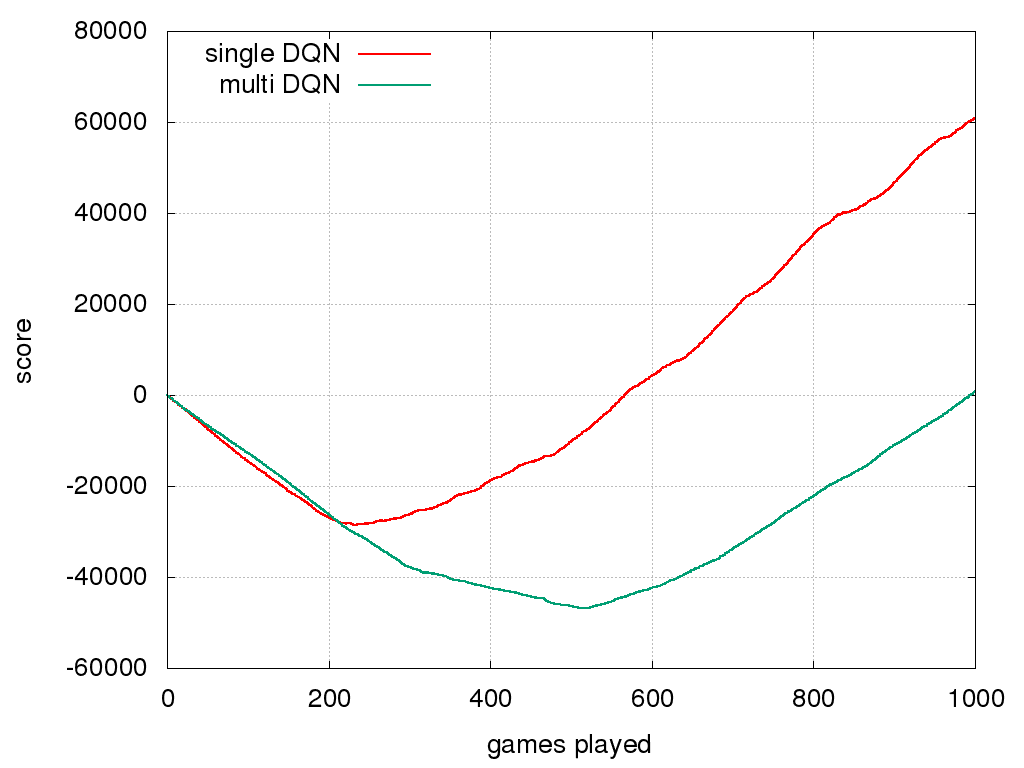
\includegraphics[width=5cm]{results/progress_training_pong.png}}\hfil
    \subfloat[Snake]{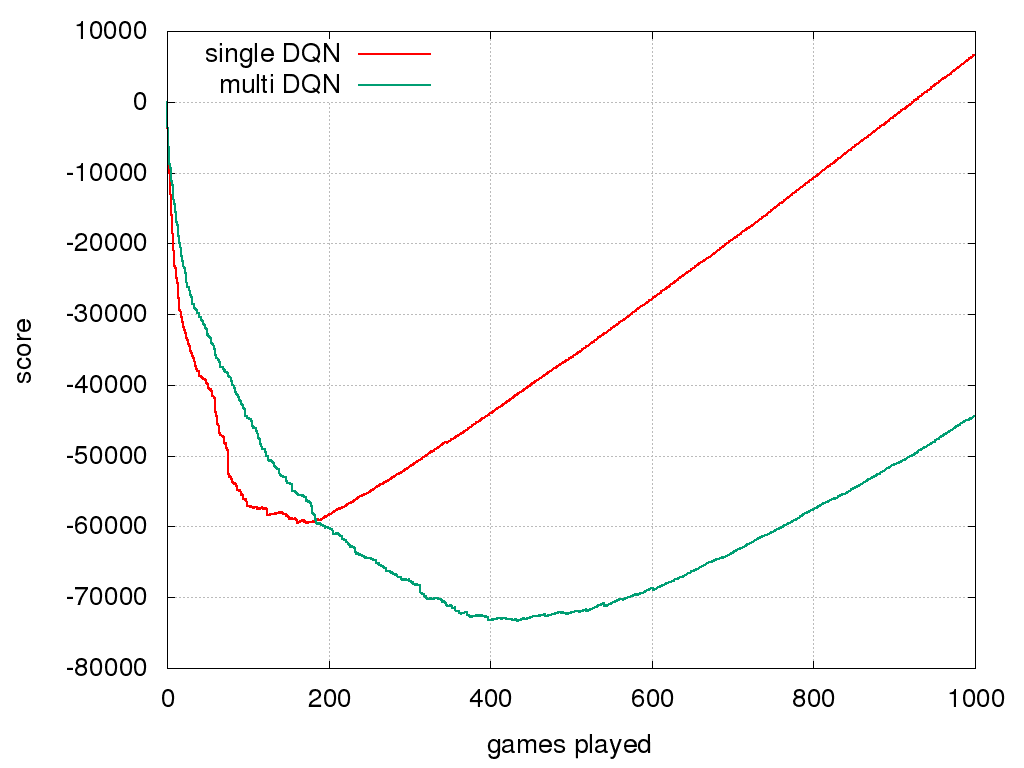
\includegraphics[width=5cm]{results/progress_training_snake.png}}
    \caption{Training score result for first 1000 games}\label{img:score_result}
\end{figure}


\begin{figure}[htb!]
\centering
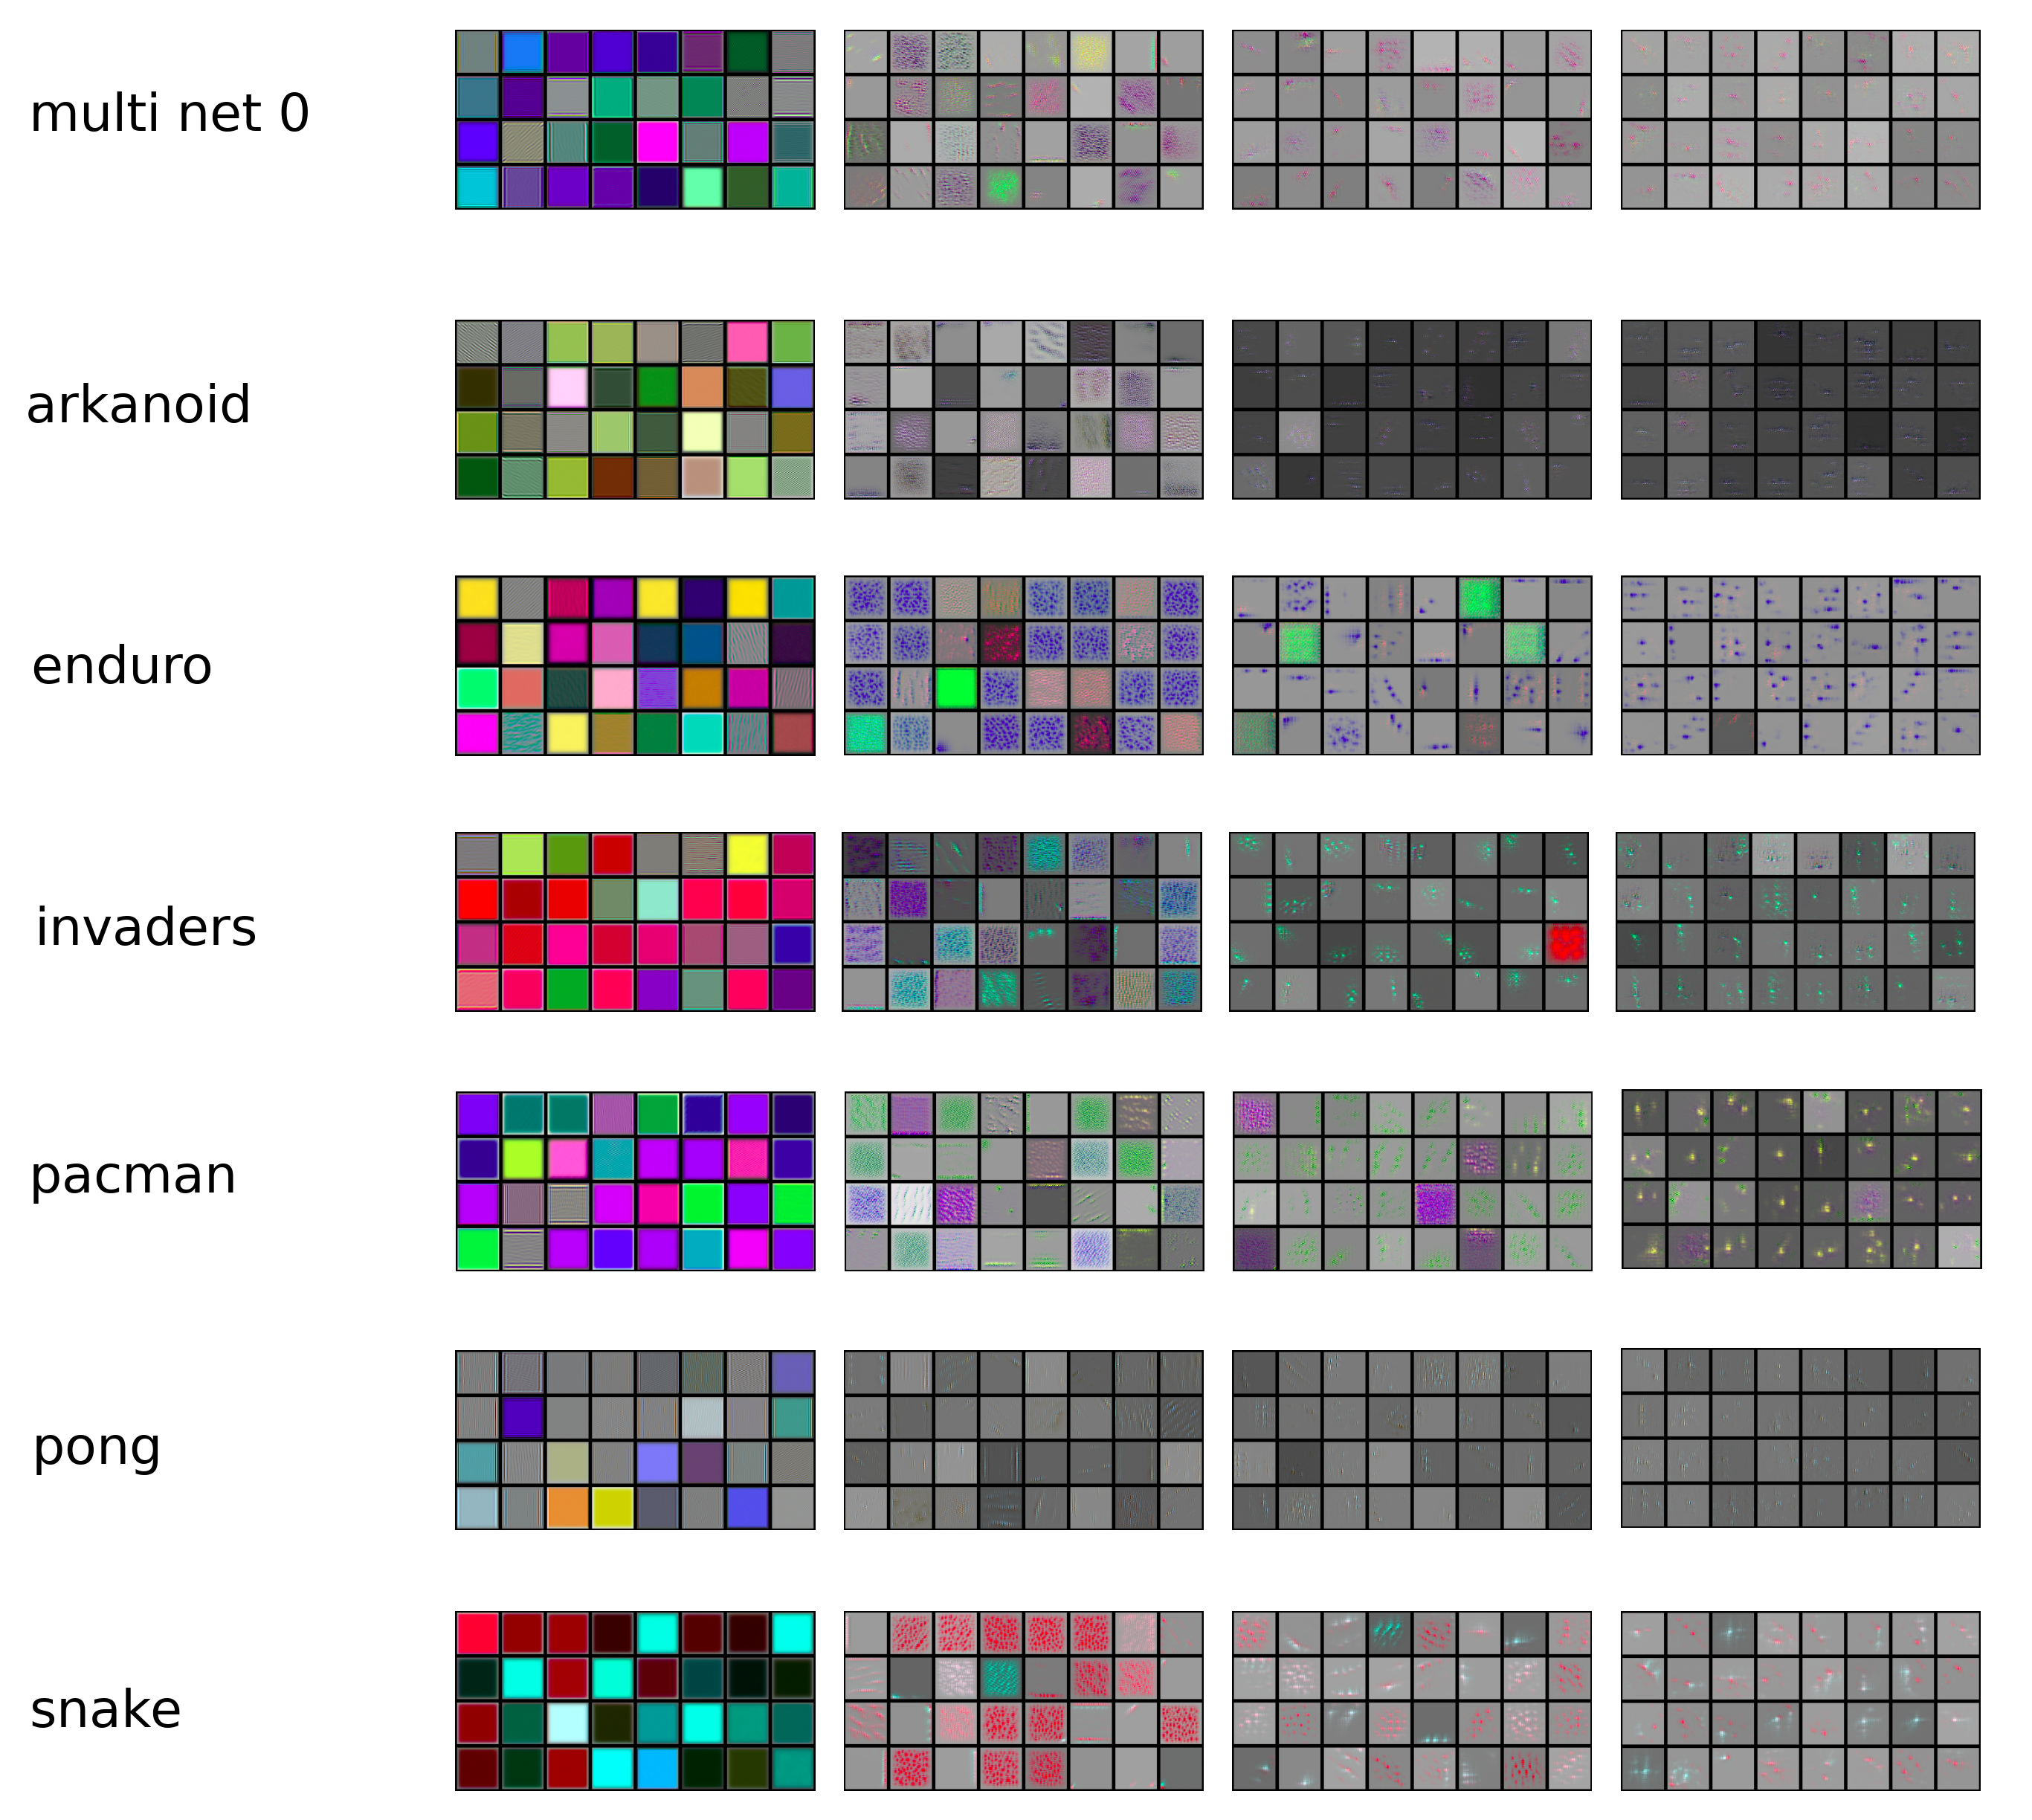
\includegraphics[width=0.7\textwidth]{results/activity/kernel_features_desc.png}
\caption{Kernel maximum response inputs visualisation for different networks}\label{img:max_response}
\end{figure}


\iffalse

\begin{figure}[htb!]
    \centering
    \subfloat[Single DQN max activity]{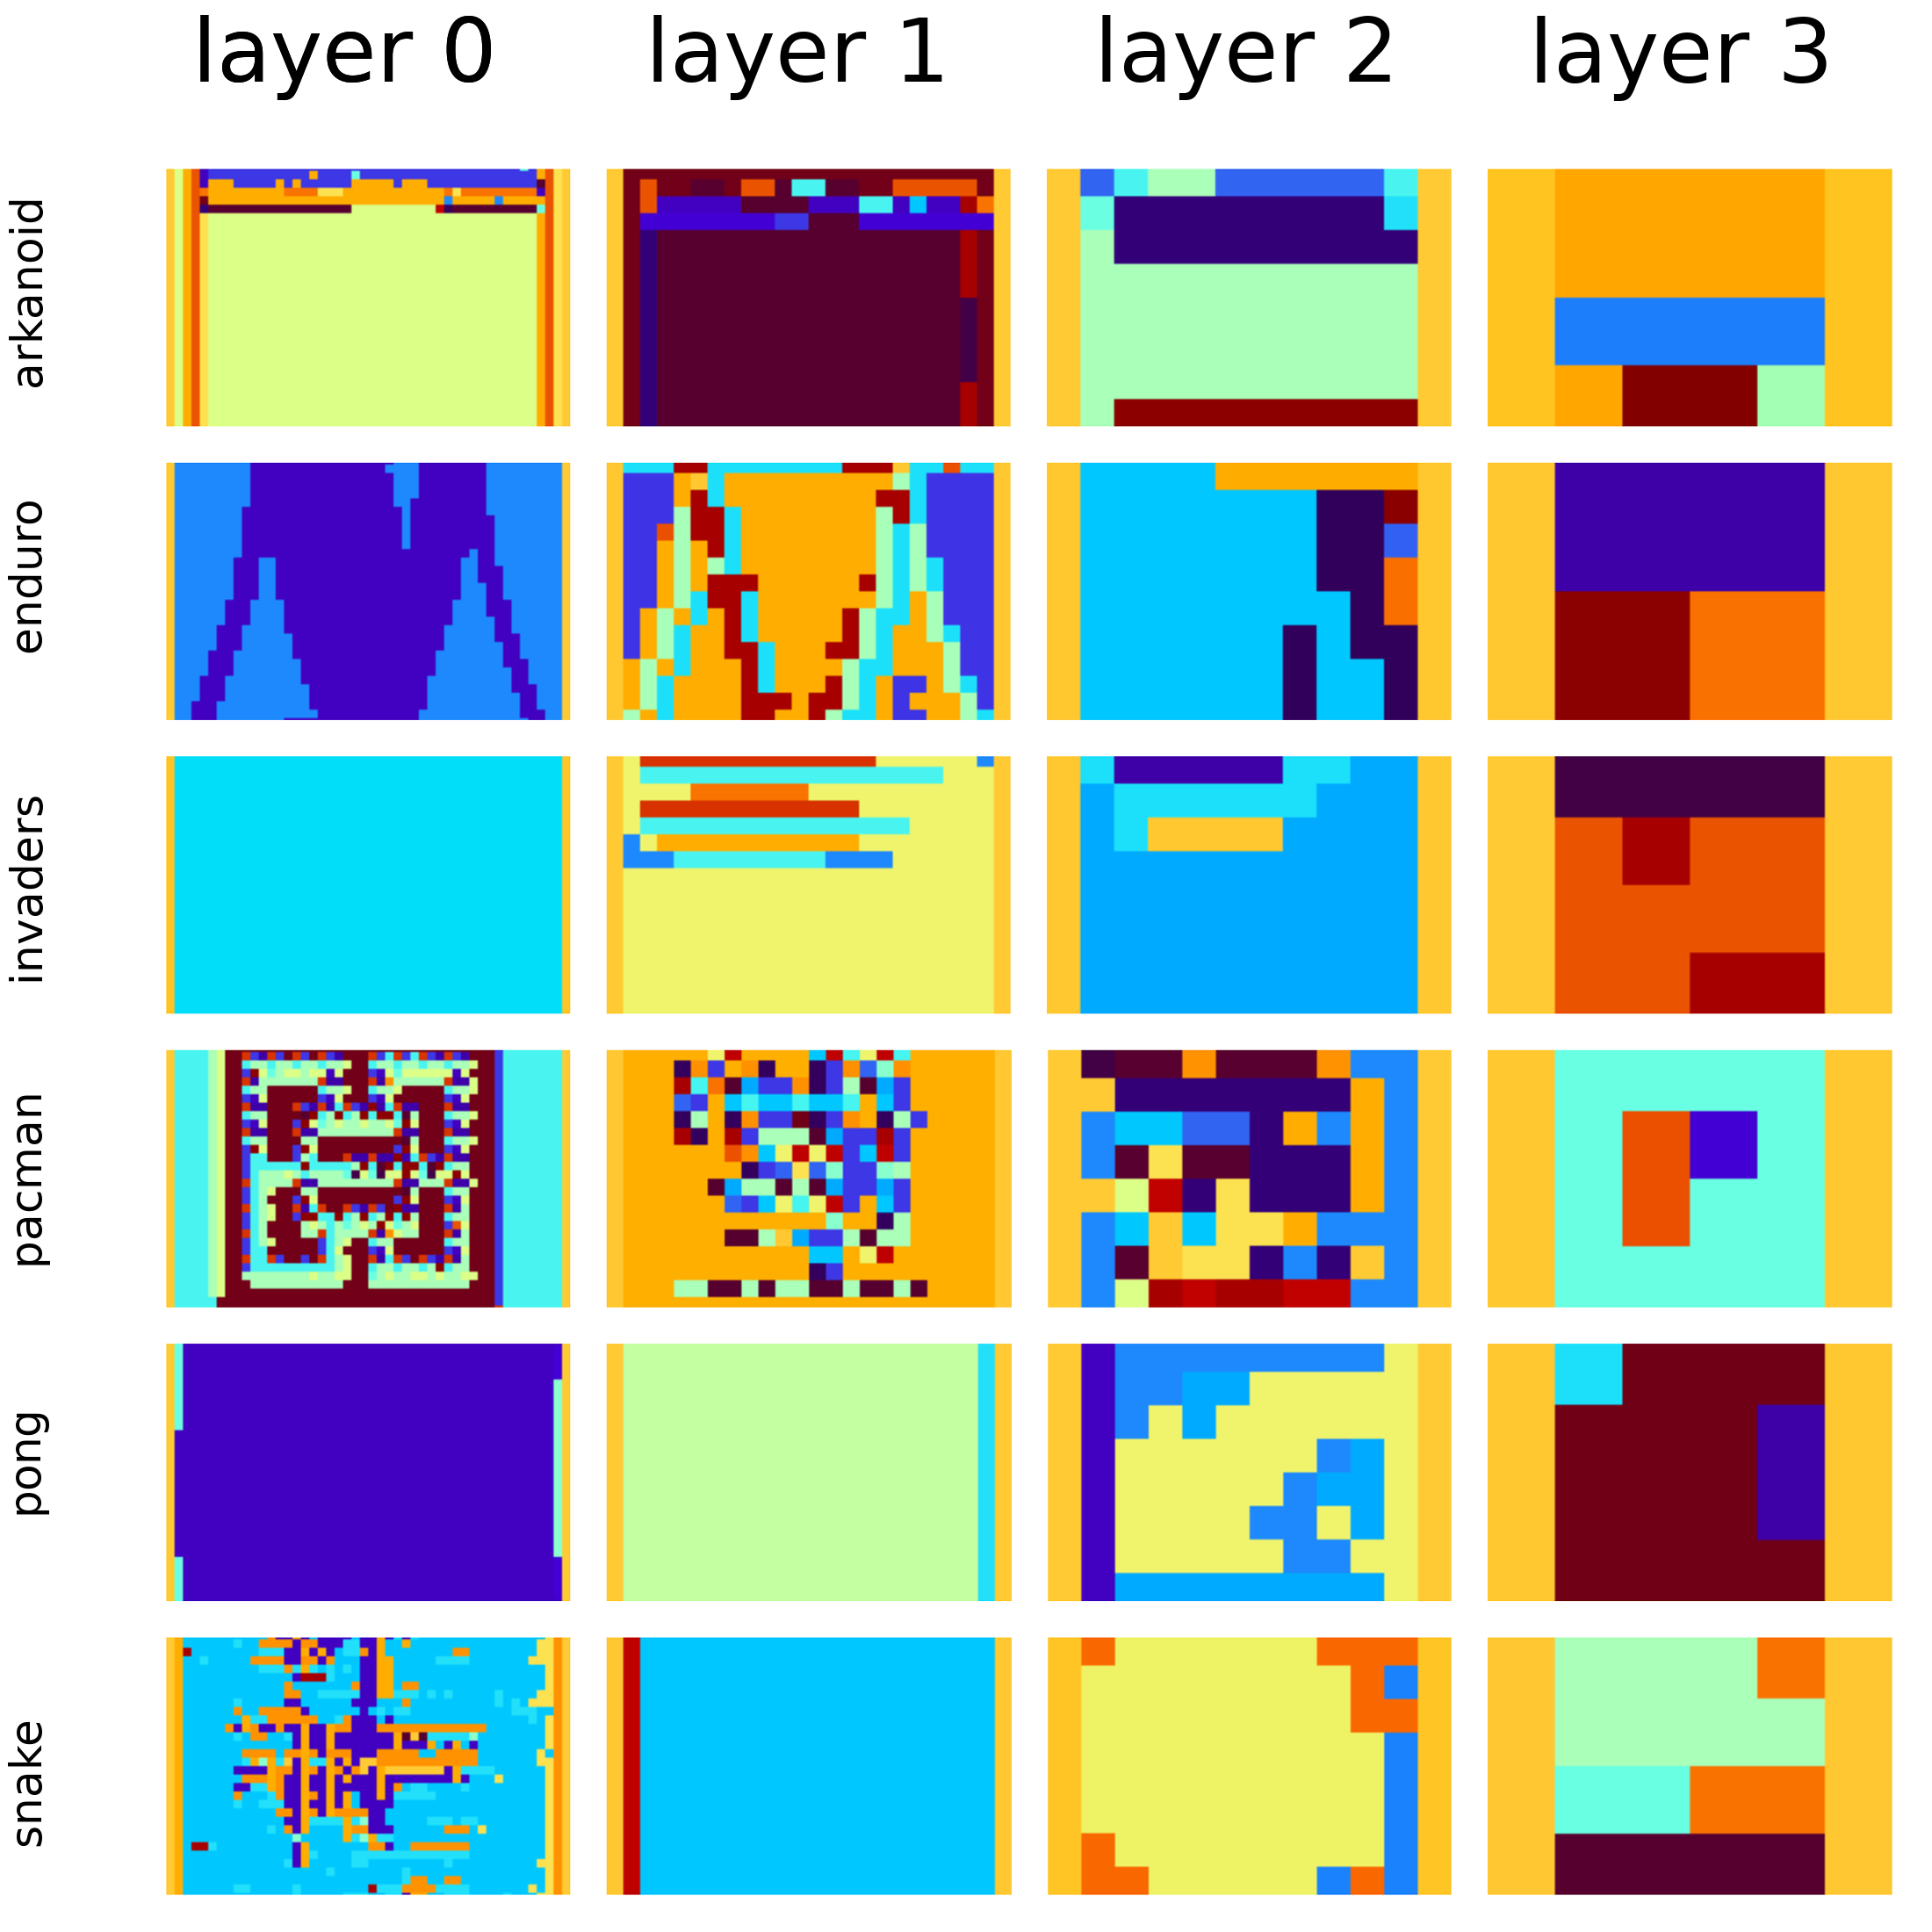
\includegraphics[width=6cm]{results/activity/single_net_max_desc.png}}\hfil
    \subfloat[Multi DQN max activity]{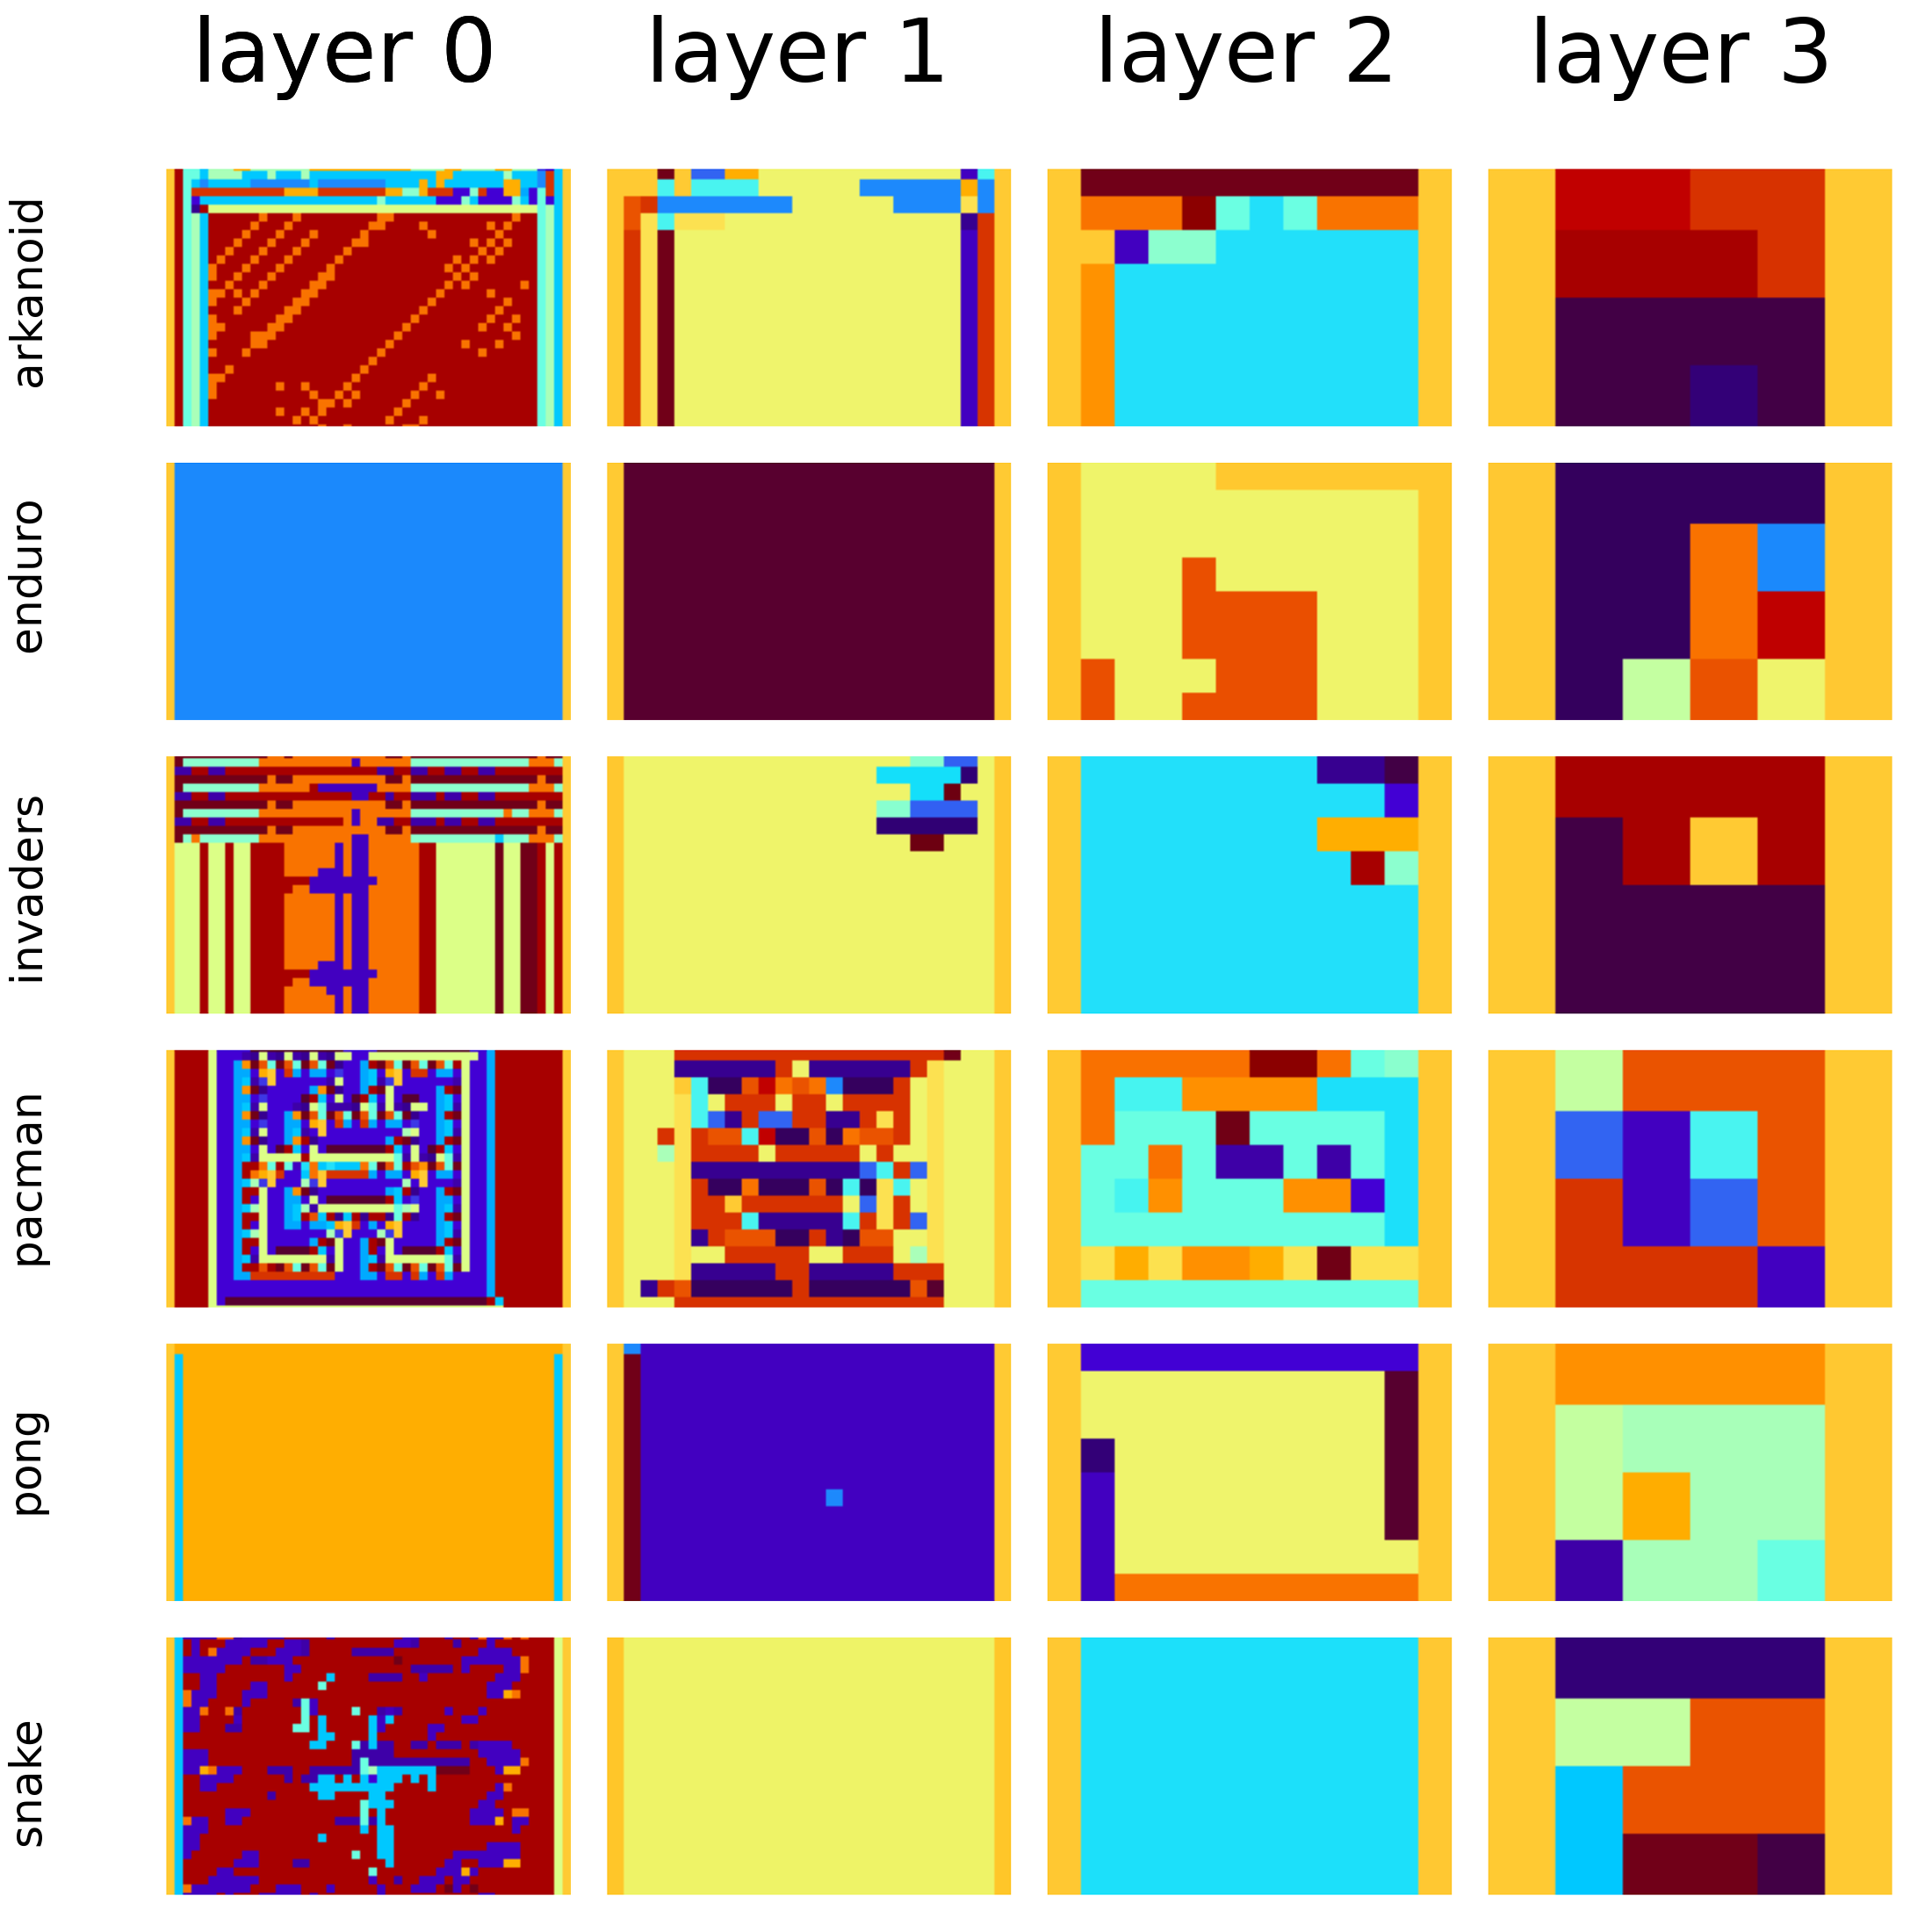
\includegraphics[width=6cm]{results/activity/multi_net0_max_desc.png}}\hfil

    \subfloat[Single DQN average activity]{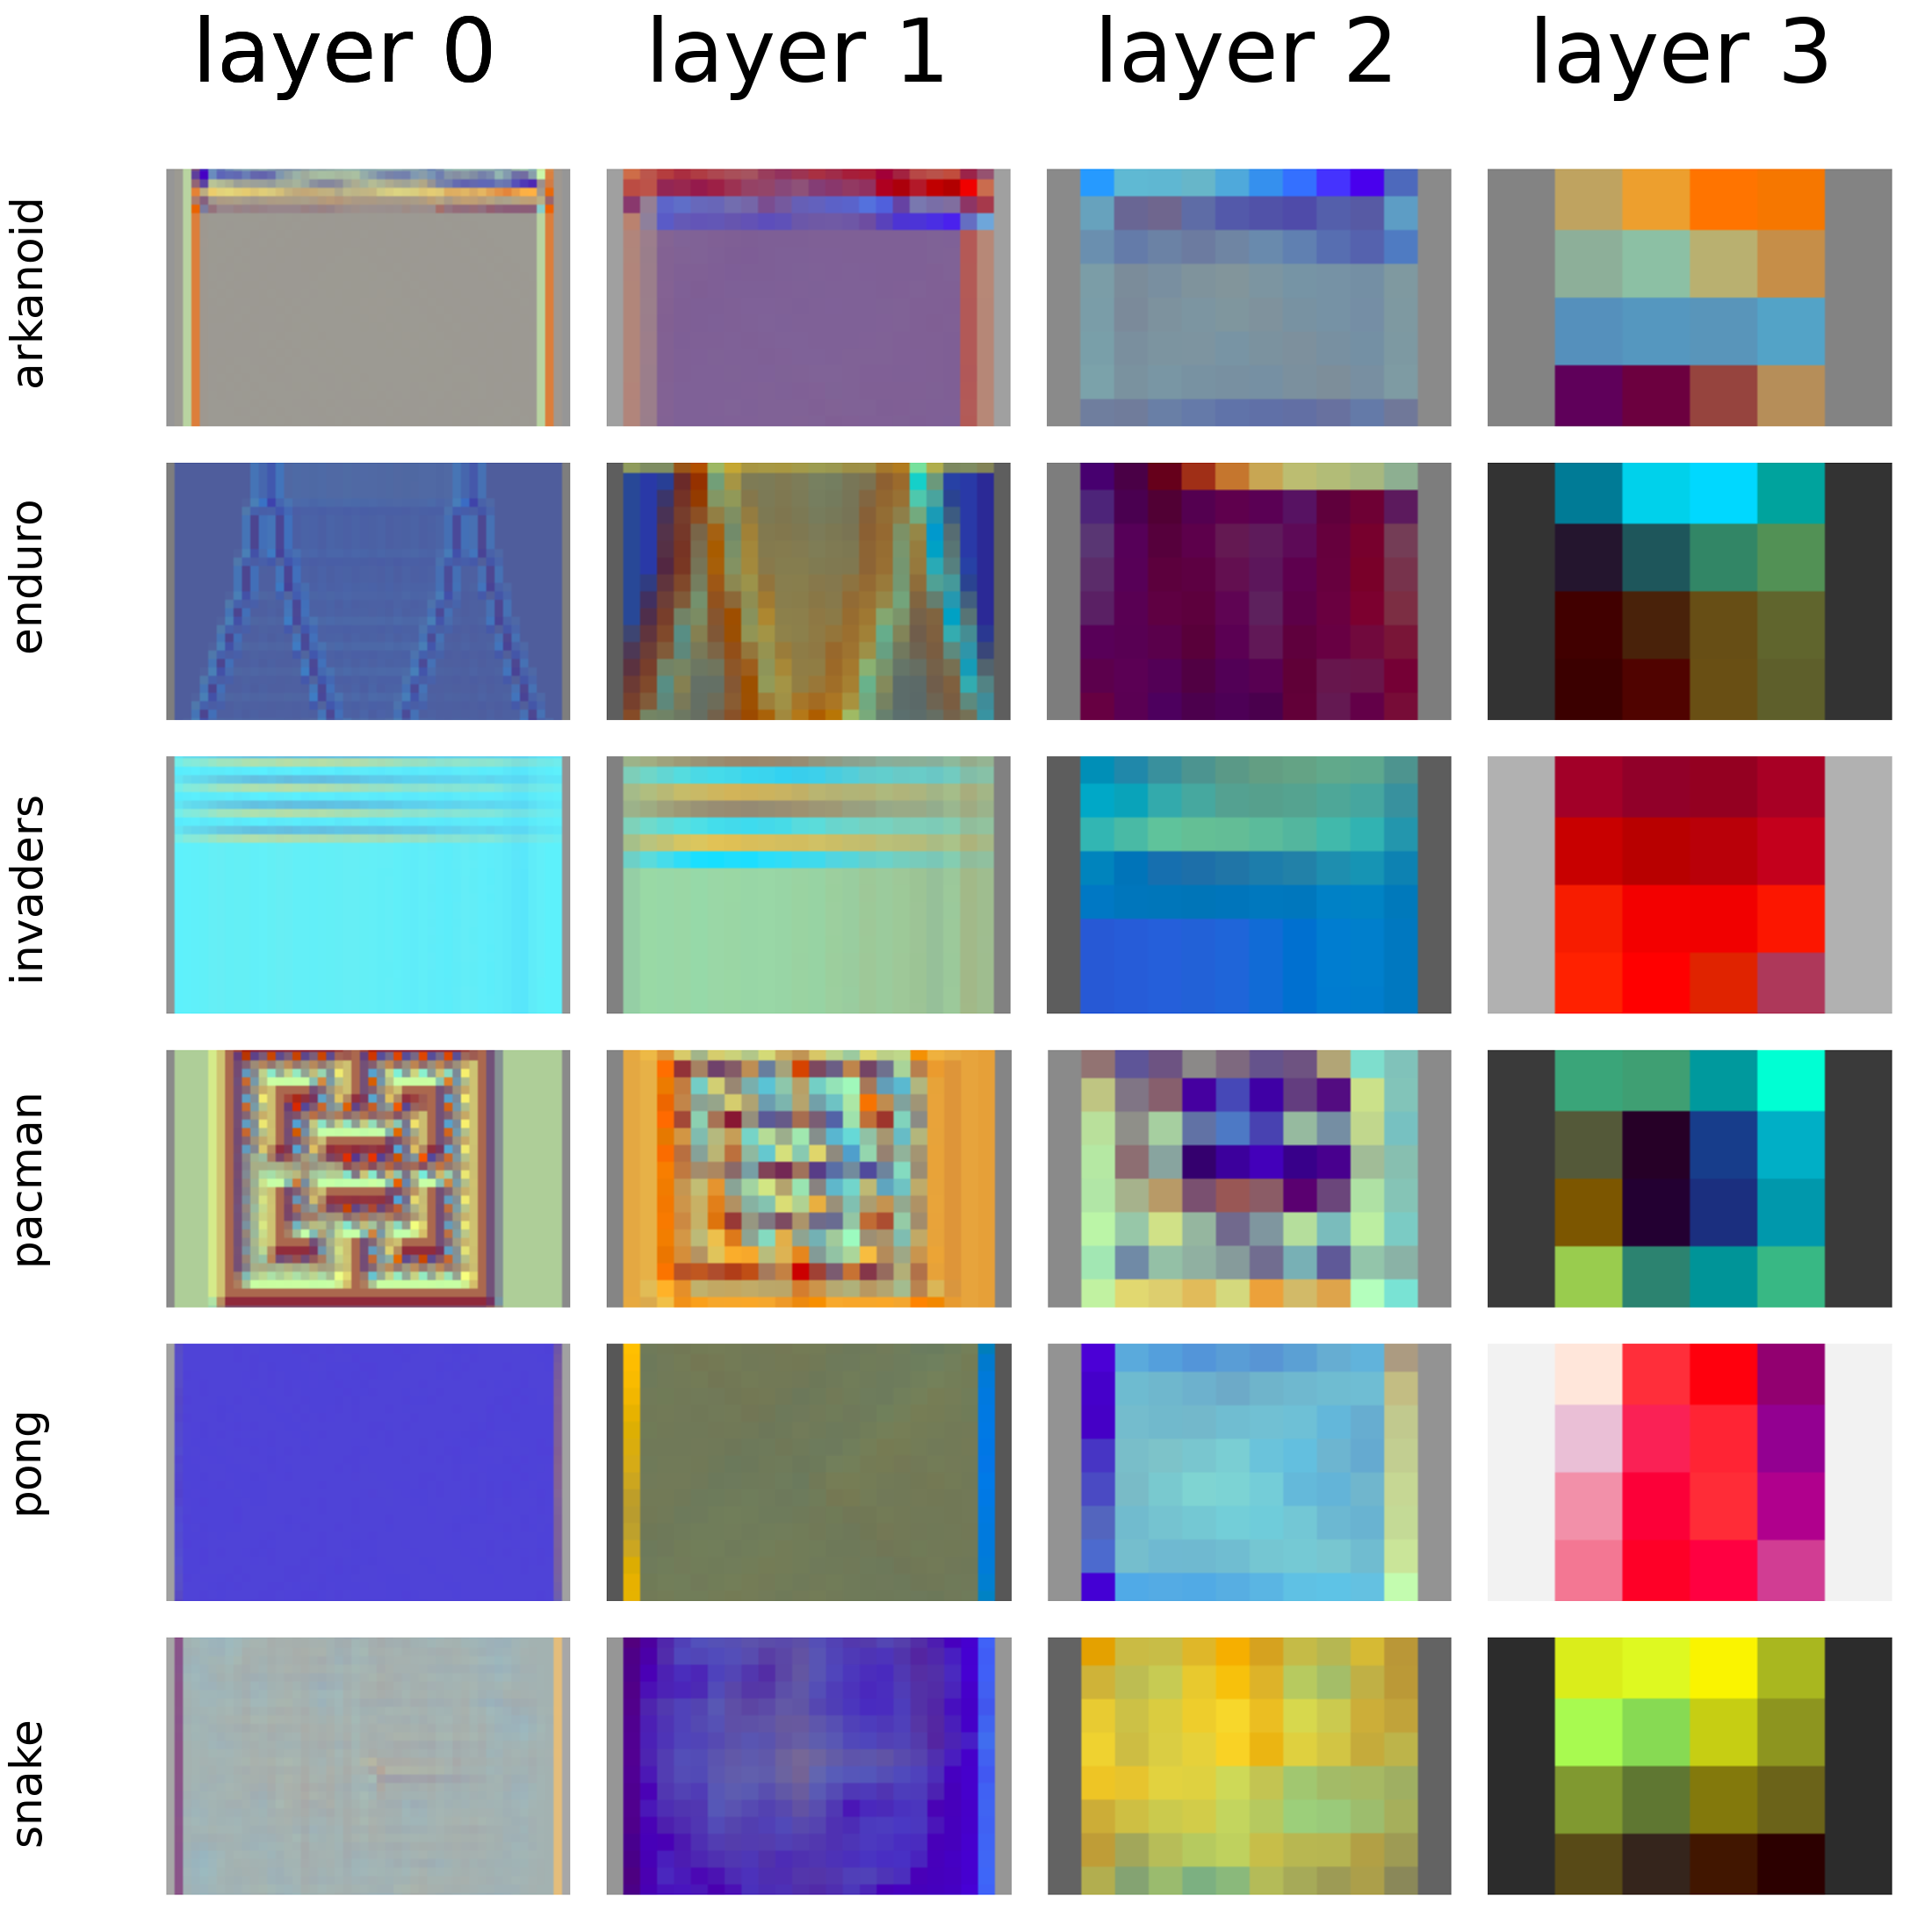
\includegraphics[width=6cm]{results/activity/single_net_average_desc.png}}\hfil
    \subfloat[Multi DQN average activity]{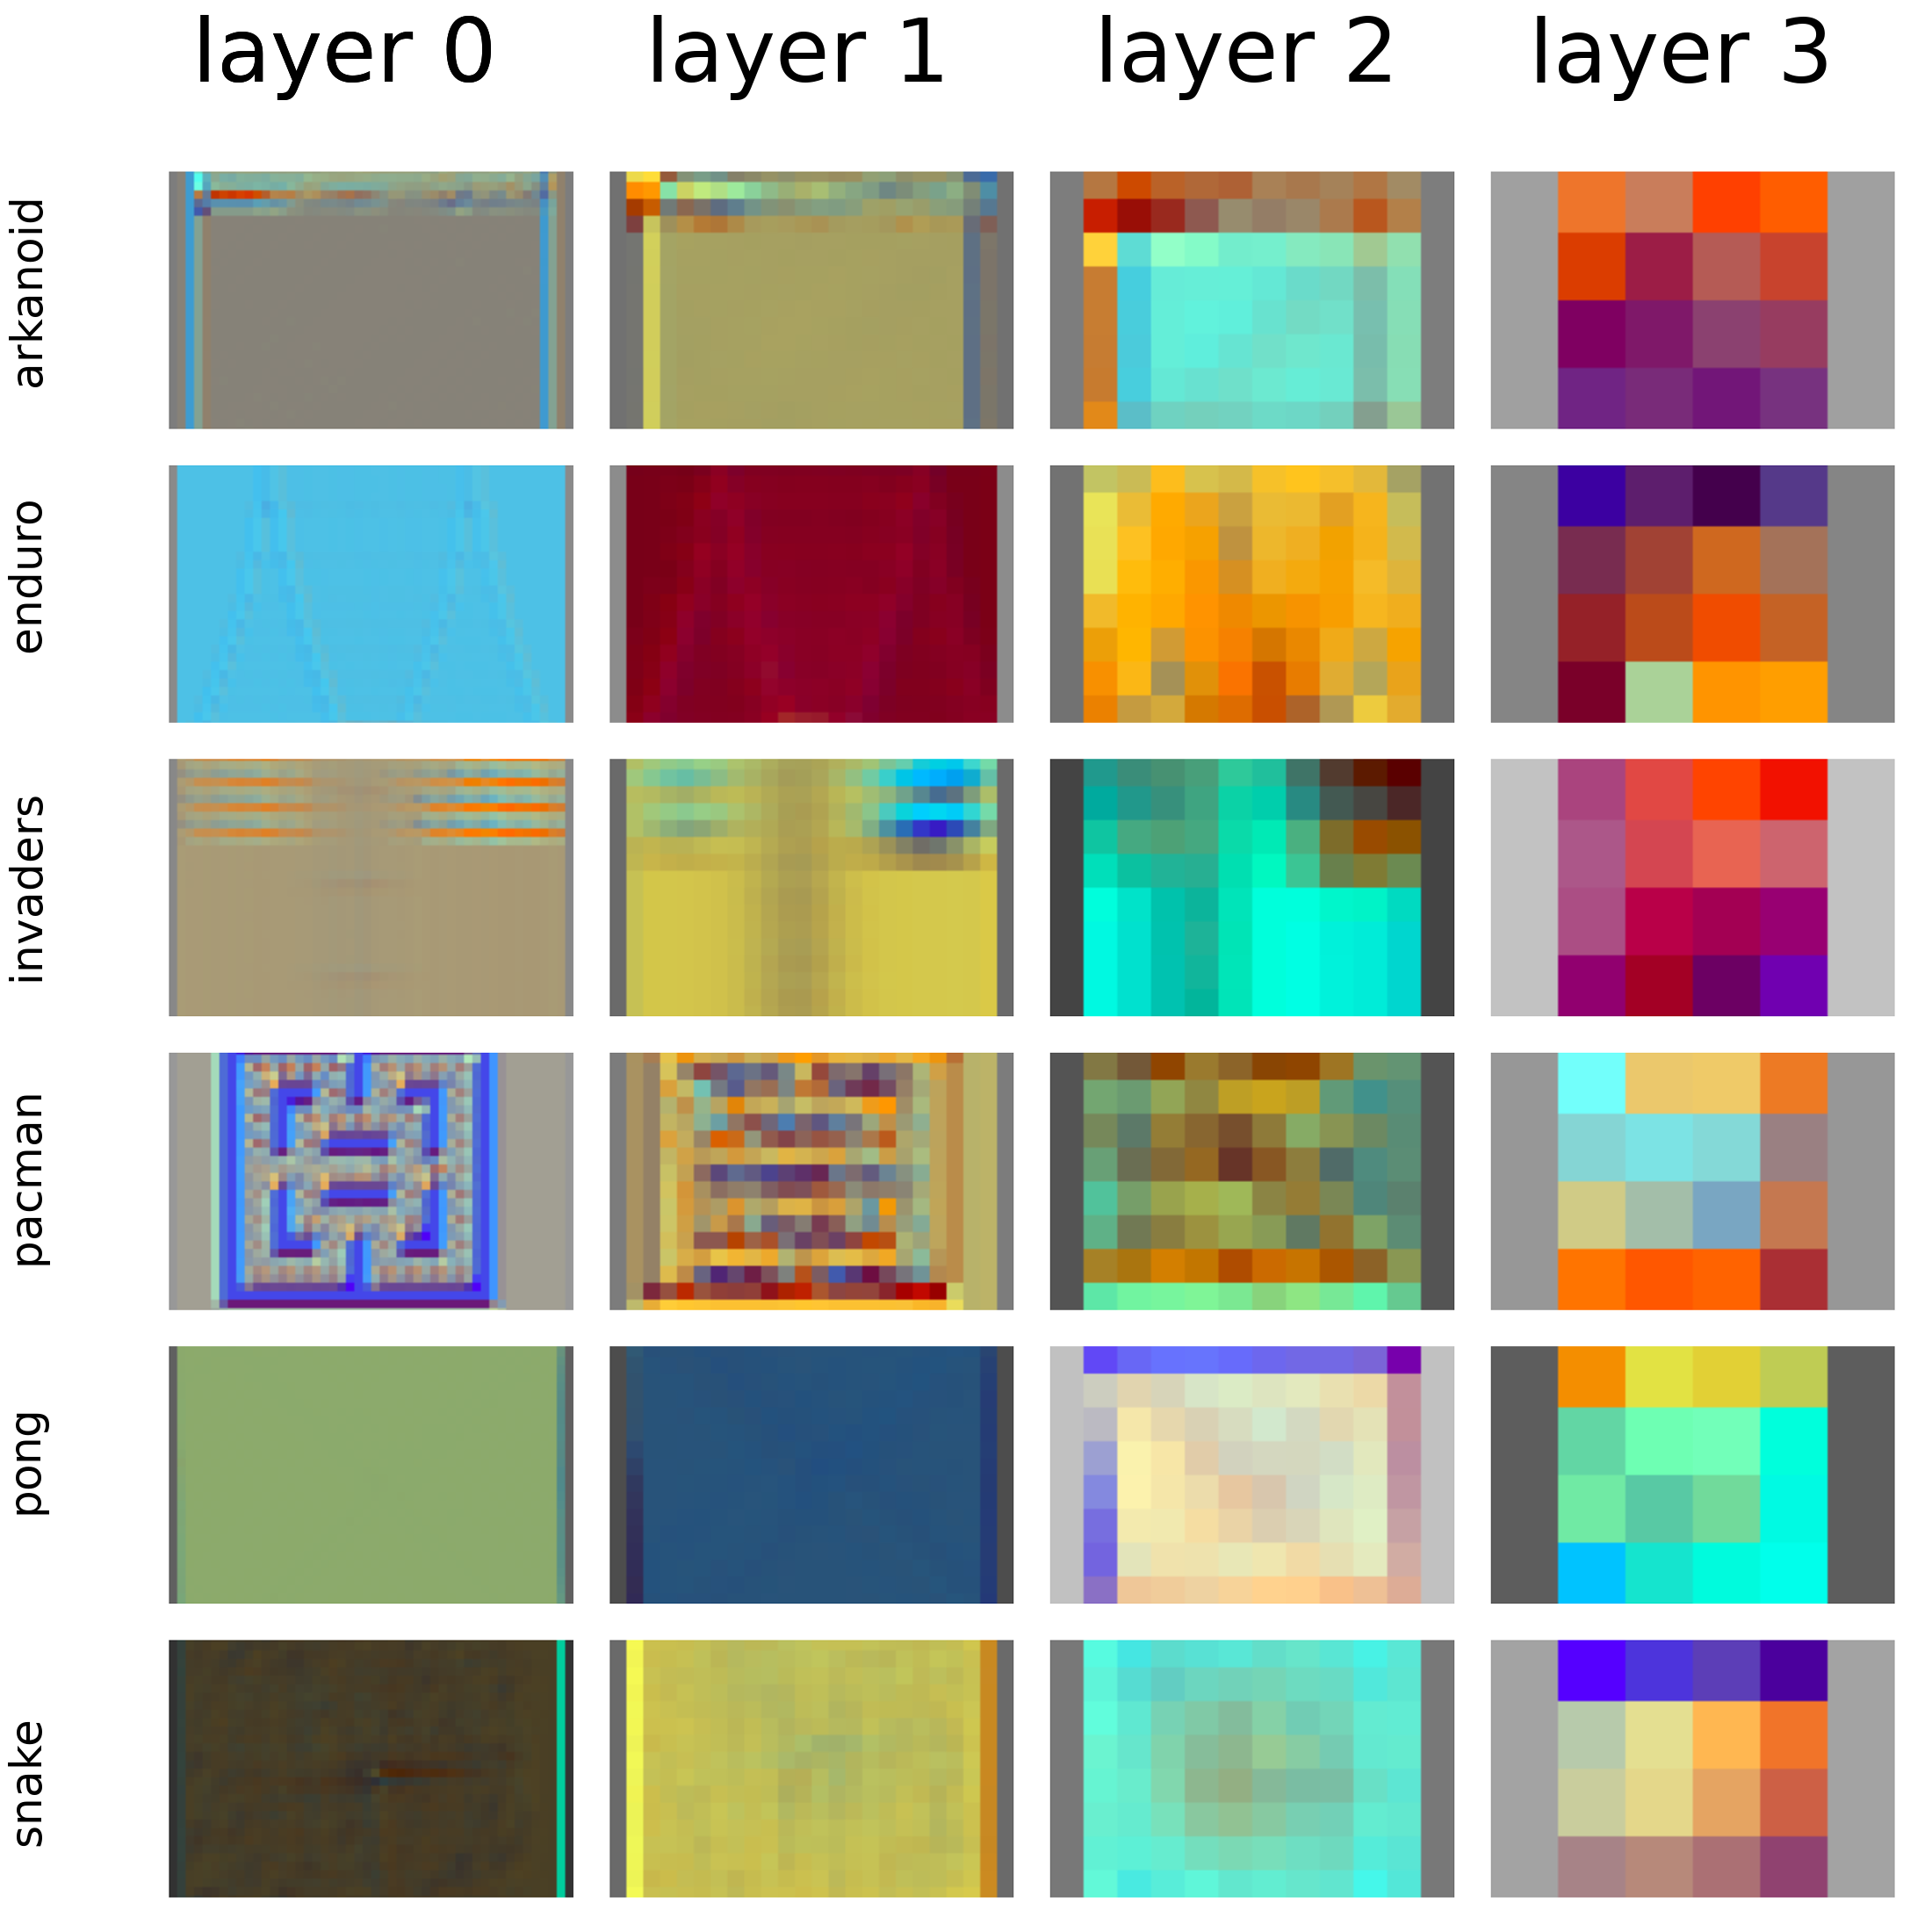
\includegraphics[width=6cm]{results/activity/multi_net0_average_desc.png}}\hfil

    \caption{Feature maps activity}\label{img:activity}
\end{figure}
\fi



\begin{table}[htb!]
\begin{tabular}{|l|c|c|c|c|c|c|c|l|}
\hline
\textbf{network}       & \textbf{arkanoid} & \textbf{enduro} & \textbf{invaders} & \textbf{pacman} & \textbf{pong} & \textbf{snake} & \textbf{multi\_net\_0} & \textbf{summary} \\ \hline
\textbf{arkanoid}      & 1.0               & 0.152           & 0.184             & 0.177           & 0.14          & 0.172          & 0.171                  & \textbf{1.9951}  \\ \hline
\textbf{enduro}        & 0.18              & 1.0             & 0.241             & 0.252           & 0.103         & 0.169          & 0.186                  & \textbf{2.1308}  \\ \hline
\textbf{invaders}      & 0.189             & 0.205           & 1.0               & 0.203           & 0.112         & 0.164          & 0.16                   & \textbf{2.0330}  \\ \hline
\textbf{pacman}        & 0.194             & 0.232           & 0.243             & 1.0             & 0.14          & 0.17           & 0.227                  & \textbf{2.2048}  \\ \hline
\textbf{pong}          & 0.118             & 0.076           & 0.086             & 0.116           & 1.0           & 0.092          & 0.114                  & \textbf{1.6013}  \\ \hline
\textbf{snake}         & 0.223             & 0.239           & 0.208             & 0.222           & 0.154         & 1.0            & 0.268                  & \textbf{2.3137}  \\ \hline
\textbf{multi\_net\_0} & 0.166             & 0.171           & 0.155             & 0.207           & 0.127         & 0.202          & 1.0                    & \textbf{2.0283}  \\ \hline
\end{tabular}


\caption{Networks correlation}\label{tab:networks_correlation}

\end{table}




\newpage
\begin{thebibliography}{9}

\bibitem{bib:dqn_atari}
Volodymyr Mnih   Koray Kavukcuoglu   David Silver   Alex Graves   Ioannis AntonoglouDaan Wierstra   Martin Riedmiller.
Playing Atari with Deep Reinforcement Learning 2013, \url{https://www.cs.toronto.edu/~vmnih/docs/dqn.pdf}

\bibitem{bib:dqn_doom}
Guillaume Lample, Devendra Singh Chaplot.
Playing FPS Games with Deep Reinforcement Learning, 2017, \url{https://arxiv.org/abs/1609.05521}

\bibitem{bib:vgg_net}
Very Deep Convolutional Networks for Large-Scale Image Recognition.
Karen Simonyan, Andrew Zisserman, 2015, \url{https://arxiv.org/abs/1409.1556}

\bibitem{bib:resnet_net}
Deep Residual Learning for Image Recognition.
Kaiming He, Xiangyu Zhang, Shaoqing Ren, Jian Sun, 2015, \url{https://arxiv.org/abs/1512.03385}

\bibitem{bib:densenet_net}
Densely Connected Convolutional Networks
Gao Huang, Zhuang Liu, Laurens van der Maaten, Kilian Q. Weinberger, 2017, \url{https://arxiv.org/abs/1608.06993}


\bibitem{bib:cbam}
Woo, Sanghyun and Park, Jongchan and Lee, Joon-Young and So Kweon, In.
CBAM: Convolutional Block Attention Module 2018, \url{https://eccv2018.org/openaccess/content_ECCV_2018/papers/Sanghyun_Woo_Convolutional_Block_Attention_ECCV_2018_paper.pdf}


\end{thebibliography}




\end{document}
